\PassOptionsToPackage{unicode=true}{hyperref} % options for packages loaded elsewhere
\PassOptionsToPackage{hyphens}{url}
%
\documentclass[]{article}
\usepackage{lmodern}
\usepackage{amssymb,amsmath}
\usepackage{ifxetex,ifluatex}
\usepackage{fixltx2e} % provides \textsubscript
\ifnum 0\ifxetex 1\fi\ifluatex 1\fi=0 % if pdftex
  \usepackage[T1]{fontenc}
  \usepackage[utf8]{inputenc}
  \usepackage{textcomp} % provides euro and other symbols
\else % if luatex or xelatex
  \usepackage{unicode-math}
  \defaultfontfeatures{Ligatures=TeX,Scale=MatchLowercase}
\fi
% use upquote if available, for straight quotes in verbatim environments
\IfFileExists{upquote.sty}{\usepackage{upquote}}{}
% use microtype if available
\IfFileExists{microtype.sty}{%
\usepackage[]{microtype}
\UseMicrotypeSet[protrusion]{basicmath} % disable protrusion for tt fonts
}{}
\IfFileExists{parskip.sty}{%
\usepackage{parskip}
}{% else
\setlength{\parindent}{0pt}
\setlength{\parskip}{6pt plus 2pt minus 1pt}
}
\usepackage{hyperref}
\hypersetup{
            pdfborder={0 0 0},
            breaklinks=true}
\urlstyle{same}  % don't use monospace font for urls
\usepackage[margin=1in]{geometry}
\usepackage{color}
\usepackage{fancyvrb}
\newcommand{\VerbBar}{|}
\newcommand{\VERB}{\Verb[commandchars=\\\{\}]}
\DefineVerbatimEnvironment{Highlighting}{Verbatim}{commandchars=\\\{\}}
% Add ',fontsize=\small' for more characters per line
\usepackage{framed}
\definecolor{shadecolor}{RGB}{248,248,248}
\newenvironment{Shaded}{\begin{snugshade}}{\end{snugshade}}
\newcommand{\AlertTok}[1]{\textcolor[rgb]{0.94,0.16,0.16}{#1}}
\newcommand{\AnnotationTok}[1]{\textcolor[rgb]{0.56,0.35,0.01}{\textbf{\textit{#1}}}}
\newcommand{\AttributeTok}[1]{\textcolor[rgb]{0.77,0.63,0.00}{#1}}
\newcommand{\BaseNTok}[1]{\textcolor[rgb]{0.00,0.00,0.81}{#1}}
\newcommand{\BuiltInTok}[1]{#1}
\newcommand{\CharTok}[1]{\textcolor[rgb]{0.31,0.60,0.02}{#1}}
\newcommand{\CommentTok}[1]{\textcolor[rgb]{0.56,0.35,0.01}{\textit{#1}}}
\newcommand{\CommentVarTok}[1]{\textcolor[rgb]{0.56,0.35,0.01}{\textbf{\textit{#1}}}}
\newcommand{\ConstantTok}[1]{\textcolor[rgb]{0.00,0.00,0.00}{#1}}
\newcommand{\ControlFlowTok}[1]{\textcolor[rgb]{0.13,0.29,0.53}{\textbf{#1}}}
\newcommand{\DataTypeTok}[1]{\textcolor[rgb]{0.13,0.29,0.53}{#1}}
\newcommand{\DecValTok}[1]{\textcolor[rgb]{0.00,0.00,0.81}{#1}}
\newcommand{\DocumentationTok}[1]{\textcolor[rgb]{0.56,0.35,0.01}{\textbf{\textit{#1}}}}
\newcommand{\ErrorTok}[1]{\textcolor[rgb]{0.64,0.00,0.00}{\textbf{#1}}}
\newcommand{\ExtensionTok}[1]{#1}
\newcommand{\FloatTok}[1]{\textcolor[rgb]{0.00,0.00,0.81}{#1}}
\newcommand{\FunctionTok}[1]{\textcolor[rgb]{0.00,0.00,0.00}{#1}}
\newcommand{\ImportTok}[1]{#1}
\newcommand{\InformationTok}[1]{\textcolor[rgb]{0.56,0.35,0.01}{\textbf{\textit{#1}}}}
\newcommand{\KeywordTok}[1]{\textcolor[rgb]{0.13,0.29,0.53}{\textbf{#1}}}
\newcommand{\NormalTok}[1]{#1}
\newcommand{\OperatorTok}[1]{\textcolor[rgb]{0.81,0.36,0.00}{\textbf{#1}}}
\newcommand{\OtherTok}[1]{\textcolor[rgb]{0.56,0.35,0.01}{#1}}
\newcommand{\PreprocessorTok}[1]{\textcolor[rgb]{0.56,0.35,0.01}{\textit{#1}}}
\newcommand{\RegionMarkerTok}[1]{#1}
\newcommand{\SpecialCharTok}[1]{\textcolor[rgb]{0.00,0.00,0.00}{#1}}
\newcommand{\SpecialStringTok}[1]{\textcolor[rgb]{0.31,0.60,0.02}{#1}}
\newcommand{\StringTok}[1]{\textcolor[rgb]{0.31,0.60,0.02}{#1}}
\newcommand{\VariableTok}[1]{\textcolor[rgb]{0.00,0.00,0.00}{#1}}
\newcommand{\VerbatimStringTok}[1]{\textcolor[rgb]{0.31,0.60,0.02}{#1}}
\newcommand{\WarningTok}[1]{\textcolor[rgb]{0.56,0.35,0.01}{\textbf{\textit{#1}}}}
\usepackage{graphicx,grffile}
\makeatletter
\def\maxwidth{\ifdim\Gin@nat@width>\linewidth\linewidth\else\Gin@nat@width\fi}
\def\maxheight{\ifdim\Gin@nat@height>\textheight\textheight\else\Gin@nat@height\fi}
\makeatother
% Scale images if necessary, so that they will not overflow the page
% margins by default, and it is still possible to overwrite the defaults
% using explicit options in \includegraphics[width, height, ...]{}
\setkeys{Gin}{width=\maxwidth,height=\maxheight,keepaspectratio}
\setlength{\emergencystretch}{3em}  % prevent overfull lines
\providecommand{\tightlist}{%
  \setlength{\itemsep}{0pt}\setlength{\parskip}{0pt}}
\setcounter{secnumdepth}{0}
% Redefines (sub)paragraphs to behave more like sections
\ifx\paragraph\undefined\else
\let\oldparagraph\paragraph
\renewcommand{\paragraph}[1]{\oldparagraph{#1}\mbox{}}
\fi
\ifx\subparagraph\undefined\else
\let\oldsubparagraph\subparagraph
\renewcommand{\subparagraph}[1]{\oldsubparagraph{#1}\mbox{}}
\fi

% set default figure placement to htbp
\makeatletter
\def\fps@figure{htbp}
\makeatother


\author{}
\date{\vspace{-2.5em}}

\begin{document}

\hypertarget{statistical-inference-course-project-part-1}{%
\section{Statistical Inference Course Project Part
1}\label{statistical-inference-course-project-part-1}}

\emph{by Szymon Tomczyk}

\begin{Shaded}
\begin{Highlighting}[]
\KeywordTok{library}\NormalTok{(tidyverse)}
\KeywordTok{library}\NormalTok{(datasets)}
\end{Highlighting}
\end{Shaded}

\hypertarget{part-1-simulation-exercise}{%
\subsection{Part 1: Simulation
Exercise}\label{part-1-simulation-exercise}}

\emph{In this part we are supposed to generate 1000 averages of 40
random exponentials from a continous exponential distribution with rate
lambda = 0.2. We will use this data to test the assumptions of LLN and
CLT in practice.}

\hypertarget{simulation}{%
\subsubsection{Simulation}\label{simulation}}

Declare the simulation parameters

\begin{Shaded}
\begin{Highlighting}[]
\KeywordTok{set.seed}\NormalTok{(}\DecValTok{666}\NormalTok{)}
\NormalTok{n <-}\StringTok{ }\DecValTok{1000}
\NormalTok{lambda <-}\StringTok{ }\FloatTok{0.2}
\end{Highlighting}
\end{Shaded}

Simulated 1000 averages of 40 exponentials from the expponential
distribution with the rate lambda = 0.2

\begin{Shaded}
\begin{Highlighting}[]
\NormalTok{s.mean =}\StringTok{ }\OtherTok{NULL}
\ControlFlowTok{for}\NormalTok{ (i }\ControlFlowTok{in} \DecValTok{1} \OperatorTok{:}\StringTok{ }\NormalTok{n) \{ s.mean <-}\StringTok{ }\KeywordTok{c}\NormalTok{(s.mean, }\KeywordTok{mean}\NormalTok{(}\KeywordTok{rexp}\NormalTok{(}\DecValTok{40}\NormalTok{, lambda))) \}}

\KeywordTok{head}\NormalTok{(s.mean)}
\end{Highlighting}
\end{Shaded}

\begin{verbatim}
## [1] 4.267297 3.640230 5.646912 4.717544 4.463866 4.974047
\end{verbatim}

\hypertarget{theoretical-statistics-vs.sample-statistics}{%
\subsubsection{Theoretical statistics vs.~sample
statistics}\label{theoretical-statistics-vs.sample-statistics}}

Calculate the theoretical mean and sample mean

\begin{Shaded}
\begin{Highlighting}[]
\DecValTok{1}\OperatorTok{/}\NormalTok{lambda }\CommentTok{## Theoretical mean}
\end{Highlighting}
\end{Shaded}

\begin{verbatim}
## [1] 5
\end{verbatim}

\begin{Shaded}
\begin{Highlighting}[]
\KeywordTok{mean}\NormalTok{(s.mean) }\CommentTok{## Sample mean}
\end{Highlighting}
\end{Shaded}

\begin{verbatim}
## [1] 4.987818
\end{verbatim}

Calculate the theoretical variance and sample variance

\begin{Shaded}
\begin{Highlighting}[]
\NormalTok{(}\DecValTok{1}\OperatorTok{/}\NormalTok{lambda}\OperatorTok{/}\KeywordTok{sqrt}\NormalTok{(}\DecValTok{40}\NormalTok{))}\OperatorTok{^}\DecValTok{2} \CommentTok{# Theoretical variance}
\end{Highlighting}
\end{Shaded}

\begin{verbatim}
## [1] 0.625
\end{verbatim}

\begin{Shaded}
\begin{Highlighting}[]
\KeywordTok{var}\NormalTok{(s.mean) }\CommentTok{# Sample variance}
\end{Highlighting}
\end{Shaded}

\begin{verbatim}
## [1] 0.6646822
\end{verbatim}

\textbf{Conclusion: both sample mean and variance are very close to the
predicted theoretical parameters. This result is in accordance with Law
of Large Numbers}

\hypertarget{normality-of-the-sampling-distribution-of-the-sampling-mean}{%
\subsubsection{Normality of the sampling distribution of the sampling
mean}\label{normality-of-the-sampling-distribution-of-the-sampling-mean}}

Plot the histogram of the sampling distribution of the mean. The red
dashed line corresponds to the theoretical mean and the grean one to the
sample mean.

\begin{Shaded}
\begin{Highlighting}[]
\NormalTok{s.mean <-}\StringTok{ }\KeywordTok{as.data.frame}\NormalTok{(s.mean)}
\NormalTok{plot <-}\StringTok{ }\KeywordTok{ggplot}\NormalTok{(s.mean, }\KeywordTok{aes}\NormalTok{(s.mean)) }\OperatorTok{+}\StringTok{ }
\StringTok{        }\KeywordTok{geom_histogram}\NormalTok{(}\KeywordTok{aes}\NormalTok{(}\DataTypeTok{y=}\NormalTok{..density..), }\DataTypeTok{bins =} \DecValTok{60}\NormalTok{, }
                       \DataTypeTok{colour =} \StringTok{"black"}\NormalTok{, }\DataTypeTok{fill =} \StringTok{"lightblue"}\NormalTok{)}\OperatorTok{+}
\StringTok{        }\KeywordTok{geom_density}\NormalTok{()}\OperatorTok{+}
\StringTok{        }\KeywordTok{geom_vline}\NormalTok{(}\KeywordTok{aes}\NormalTok{(}\DataTypeTok{xintercept=}\KeywordTok{c}\NormalTok{(}\DecValTok{1}\OperatorTok{/}\NormalTok{lambda)),  }
                   \DataTypeTok{color=}\StringTok{"red"}\NormalTok{, }\DataTypeTok{linetype=}\StringTok{"dashed"}\NormalTok{, }
                   \DataTypeTok{size =} \FloatTok{0.5}\NormalTok{)}\OperatorTok{+}\StringTok{ }
\StringTok{        }\KeywordTok{geom_vline}\NormalTok{(}\KeywordTok{aes}\NormalTok{(}\DataTypeTok{xintercept=}\KeywordTok{mean}\NormalTok{(s.mean)),  }
                   \DataTypeTok{color=}\StringTok{"green"}\NormalTok{, }\DataTypeTok{linetype=}\StringTok{"dashed"}\NormalTok{, }
                   \DataTypeTok{size =} \FloatTok{0.5}\NormalTok{)}\OperatorTok{+}\StringTok{ }
\StringTok{        }\KeywordTok{xlab}\NormalTok{(}\StringTok{"Mean"}\NormalTok{) }\OperatorTok{+}\StringTok{ }\KeywordTok{ylab}\NormalTok{(}\StringTok{"Frequency"}\NormalTok{)}
\NormalTok{plot}
\end{Highlighting}
\end{Shaded}

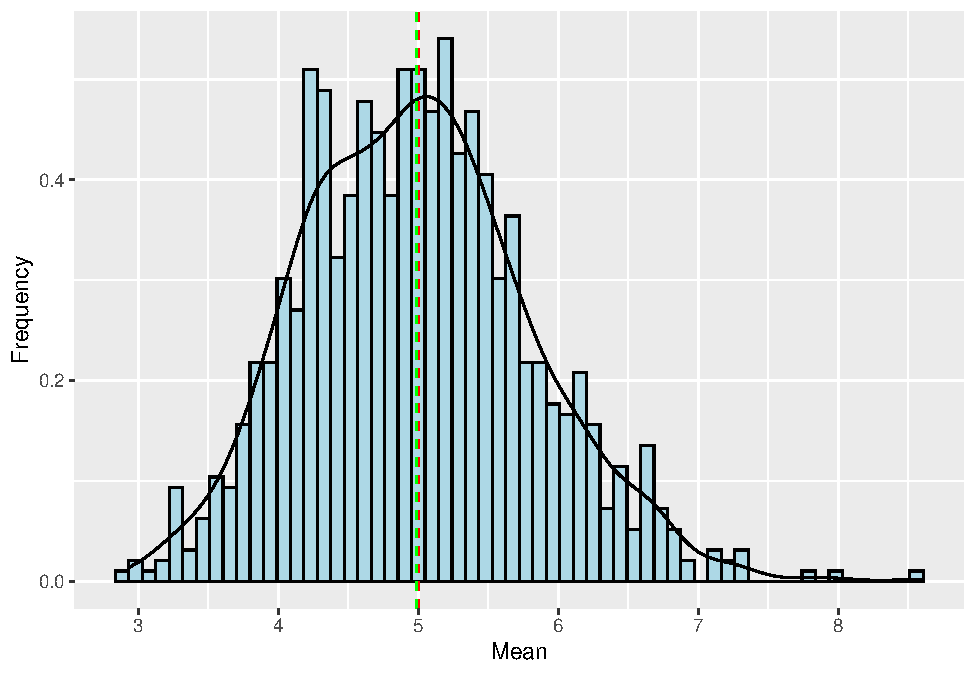
\includegraphics{IS_final_assignment_part1_files/figure-latex/unnamed-chunk-6-1.pdf}

Test with Shapiro--Wilk test for normality

\begin{Shaded}
\begin{Highlighting}[]
\KeywordTok{shapiro.test}\NormalTok{(s.mean}\OperatorTok{$}\NormalTok{s.mean)}
\end{Highlighting}
\end{Shaded}

\begin{verbatim}
## 
##  Shapiro-Wilk normality test
## 
## data:  s.mean$s.mean
## W = 0.99187, p-value = 2.584e-05
\end{verbatim}

\textbf{Conclusion: Under the CLT we can assume that the sampling
distribution of the mean is approximately normal. However, our specific
sample does not pass Shapiro--Wilk test so the normality assumtion is
not valid.}

\end{document}
